% !TEX root =  paper.tex
\section{Biologically-Constrained Error Correction}

\begin{figure*}[t!]
	\centering
	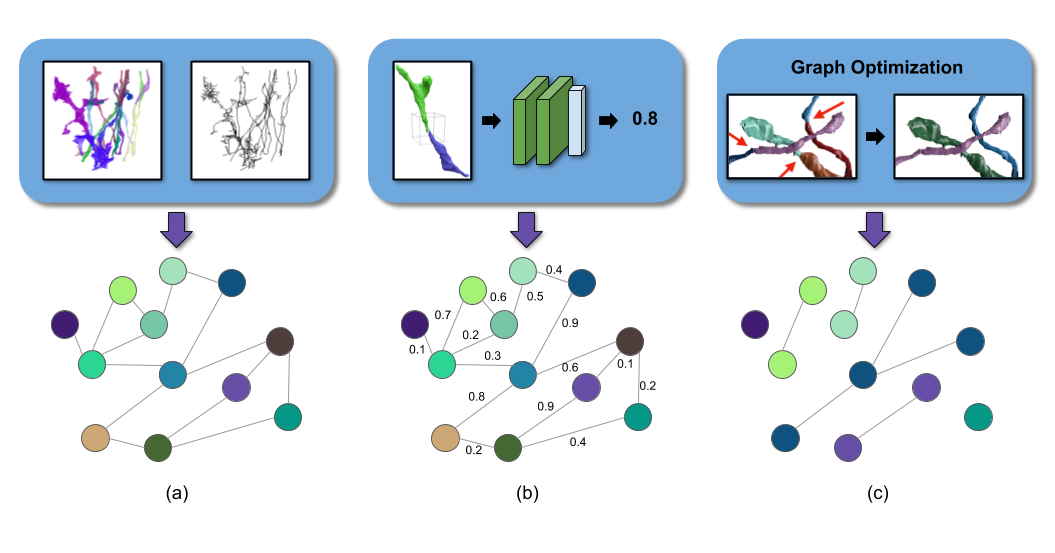
\includegraphics[width=0.75\linewidth]{./figures/teaser_v4.png}
	\caption{Our framework uses both geometric and topological biological constraints for region merging. We (a) generate a simplified graph from the skeleton representation of the input segmentation, (b) train a classifier to learn the edge weight based on the shape of the segment connection, and (c) perform graph partitioning with acyclic constraints.}
	\label{fig:teaser_pipeline}
\end{figure*}

Our method is illustrated in Fig.~\ref{fig:teaser_pipeline}.
From the input segmentation we generate a graph $G$ with nodes $N$ and edges $E$ with weights $w_e$. 
The nodes correspond to labeled segments from the input data with edges between merge candidates.
We propose the following three steps to formulate and then partition the graph while obeying constraints from the underlying biology.
First, we only consider merging segments based on a skeletonized representation of the input segmentation (Fig.~\ref{fig:teaser_pipeline}a).
This enables us to reduce the number of edges in the graph based on prior knowledge on the shape of neuronal processes.
Second, we train a convolutional neural network that learns biological constraints based on the shapes of the input segmentation (Fig.~\ref{fig:teaser_pipeline}b).
This network generates probabilities that segments belong to the same neuron based only on the segmentations. 
An example of one such learned constraint is that neurons have small turning radii (Fig.~\ref{fig:turn-radii}).
Third, we partition the graph using a lifted multicut formulation with additional acyclic constraints to enforce global biological constraints (Fig.~\ref{fig:teaser_pipeline}c).
The lifted multicut solution is globally consistent which we then augment to produce a tree-structured graph.

\subsection{Skeleton-Based Graph Generation}
\label{sec:skeletonization}
Most region merging methods create a region graph by removing small-sized segments and linking each pair of adjacent segments, which can still lead to a large graph size due to the irregular shape of neural structures.
We use a skeleton representation of the segmentation to reduce the graph size with geometric constraints on the connectivity of two adjacent segments to prune edges.

Our key observation is that if two segments belong to the same neuronal process, their skeleton end points should satisfy certain geometric constraints.
To extract the skeleton from each segment, we use a variant~\cite{zhao2014automatic} of the TEASER algorithm~\cite{sato2000teasar}. 
Fig.~\ref{fig:skeletonization} shows four examples of extracted skeletons (in black). 
These skeletons consist of a sequence of \textit{joints}, locations that are locally a maximum distance from the segment boundary, with line segments connecting successive joints. 
We refer to joints that have only one connected neighbor as \textit{endpoints}. 
We find that approximately 70\% of the segments that are erroneously split have nearby endpoints (Fig.~\ref{fig:merge_candidates}). 

Two segments, $s_1$ and $s_2$, receive a corresponding edge if the two following conditions hold.
First, endpoints in either $s_1$ or $s_2$ are within $t_{low}$ nm of any voxel in the other segment.
Second, there are endpoints in $s_1$ and in $s_2$ that are within $t_{high}$ nm of each other.
We store the midpoints between the two endpoints as the center of the potential merge in the set $\mathbb{S}_c$. 
This algorithm produces a set of segments to consider for merging. 
Only these pairs have a corresponding edge in the constructed graph.

\subsection{Learning-based Edge Weight}
\label{sec:edge-weights}

To predict the probabilities that two segments belong to the same neuron, we train a feed-forward convolutional network with three \textit{VGG-style} convolution blocks~\cite{chatfield2014return} and two fully connected layers before the final sigmoid activation. 
For the input of the network, we extract a cubic region of interest (ROI) around each endpoint $e$ in $\mathbb{S}_c$ as input to the CNN. 
There are three channels corresponding to voxels belonging to label one, label two, or either label.
We do not use the raw EM image information to avoid the need to retrain the network on datasets that have been stained differently or imaged at different resolution. 
This reduces the need for generating costly manually-labeled ground truth. 

\subsection{Optimization-Based Graph Partition}

\label{sec:optimization}

After constructing the graph we seek to partition it into labels where every label corresponds to a neuronal process. 
We formulate this graph partitioning problem as a multicut problem.
There are two primary benefits to using a multicut formulation. 
First, the number of segments in the final graph is not predetermined but depends on the input. 
Second, this minimization produces globally consistent solutions (i.e., a boundary remains only if the two corresponding nodes belong to unique segments)~\cite{keuper2015efficient}.

We apply the algorithms of Keuper et al.~\cite{keuper2015efficient} to produce a feasible solution to the multicut problem using greedy additive edge contraction.
Following their example, we employ the generalized lifted multicut formulation.
Traditional multicut solutions only consider the probabilities that two adjacent nodes belong to the same segment. 
In the lifted extension to the problem, we can penalize non-adjacent nodes that belong to different segments. 
These penalties between non-adjacent nodes are called lifted edges. 
Ideally these lifted weights represent the probability that two nodes belong to the same neuron.
However, determining such probabilities is computationally expensive.
We approximate these probabilities by finding the maximal probable path between any two nodes using Dijkstra's algorithm~\cite{keuper2015efficient}.
This is an underestimate of the probability that two nodes belong to the same neuron since it does not consider all possible paths.
Since our graphs are sufficiently small, we can generate lifted edges between all pairs of nodes. 

We need to convert the probabilities into the following weighting scheme to solve the multicut problem with this heuristic~\cite{andres2011probabilistic,keuper2015efficient}.
Given the probability that the nodes belong to the same neuron is $p_e$, the edge weight $w_e$ is defined as
%p_e &=\mbox{CNN}(x_1, x_2) \\
\begin{align}
w_e = \log{\frac{p_e}{1 - p_e}} + \log{\frac{1 - \beta}{\beta}},
\end{align}
where $\beta$ is a tunable parameter that encourages over- or under-segmentation. 
Since, there are many more lifted edges than adjacent edges, we scale down the lifted weights proportionally to their total number  
~\cite{beier2017multicut}.

By reformulating the segmentation problem as a graph partitioning one, we can enforce some global constraints on our result based on the underlying biology.
Traditional hierarchical clustering algorithms do not rely on such constraints but consider local decisions independently.
We enforce a global constraint that neurons are tree-structured and should not contain cycles. 
The multicut problems returns a series of ``collapsed'' edges between nodes that belong to the same neuron.
We iterate over these edges in order of the probability of merge generated by our CNN. 
We ``collapse'' an edge only if it does not create a cycle in the graph.
